\documentclass[12pt,letterpaper]{article}

\usepackage[utf8]{inputenc} % OJO!!!  => MANTENER ESTA LINEA PARA FACIL CONVERSION A WORD EN EL FUTURO ...
% \usepackage[spanish]{babel}
\usepackage{graphicx} 
\usepackage{array}
\usepackage{tabularx}
\usepackage{amssymb, amsmath}

% Paquetes extras ... 
\usepackage{subfigure}
\usepackage{color}
\definecolor{mygreen}{RGB}{28,172,0} % color values Red, Green, Blue
\definecolor{mylilas}{RGB}{170,55,241}

\usepackage{hyperref}
\usepackage{enumitem}

% \usepackage[T1]{fontenc}

% \usepackage{helvet}
% \renewcommand{\familydefault}{\sfdefault}

\usepackage{amsmath,amsfonts,amssymb,amsthm,cancel,icomma,nicefrac,mathrsfs,
            eurosym,verbatim,environ,ifthen,ifdraft,pdfpages,float,booktabs}
\allowdisplaybreaks[1] 

\usepackage{color}
\definecolor{lstgrey}{rgb}{0.95,0.95,0.95}
\usepackage{listings}
\lstset{language=Matlab,
       backgroundcolor=\color{lstgrey},
       frame=single,
       basicstyle=\footnotesize\ttfamily,
       captionpos=b,
       tabsize=2,
  }

  \lstset{language=Matlab,%
  %basicstyle=\color{red},
  breaklines=true,%
  morekeywords={matlab2tikz},
  keywordstyle=\color{blue},%
  morekeywords=[2]{1}, keywordstyle=[2]{\color{black}},
  identifierstyle=\color{black},%
  stringstyle=\color{mylilas},
  commentstyle=\color{mygreen},%
  showstringspaces=false,%without this there will be a symbol in the places where there is a space
  numbers=left,%
  numberstyle={\tiny \color{black}},% size of the numbers
  numbersep=9pt, % this defines how far the numbers are from the text
  emph=[1]{for,end,break},emphstyle=[1]\color{red}, %some words to emphasise
  %emph=[2]{word1,word2}, emphstyle=[2]{style},    
}


\title{Homework 1 - Equilibria, Eigen Analysis, Simulation}
\author{Jose Eduardo Laruta Espejo \\ Facultad de Ingeniería - Universidad Mayor de San Andrés}
\begin{document}
\maketitle
\section{Finding Equilibria}

\subsection{Simulating the model}
Our plant model is given by the following ODE system:

\begin{align} 
    \dot{x_1} &= \frac{u_1}{V}(u_3 - x_1) - R \label{eq:exo1} \\
    \dot{x_2} &= \frac{u_1}{V}(u_2 - x_2) + \frac{\gamma}{\sigma}R \label{eq:exo2}
\end{align}

where $R = \alpha x_1 e^{-\frac{\beta}{x_2 + 46}}$, and the constant are: $\alpha = 3.0 \times 10^{11} min^{-1}, 
\beta = 2.8 \times 10^3 Rankin/10, \gamma = 8 BTU/klb-mole, \sigma = 5 BTU/(gal-deg F), V = 1000 gallons/10$
and constant inputs: $u_1 = 50.5, u_2 = 33.794, u_3 = 19.5037$.

The resulting code for simulating the model is as follows:

\lstinputlisting{../matlab/exo.m}

Now, we can find the two stable equilibria by simulation, with the following initial condition and function calls:
\lstinputlisting{../matlab/simu_noplot.m}

the results of simulation:

%%%% Figura 1 %%%%%%
\begin{figure}[!h] 
\centering
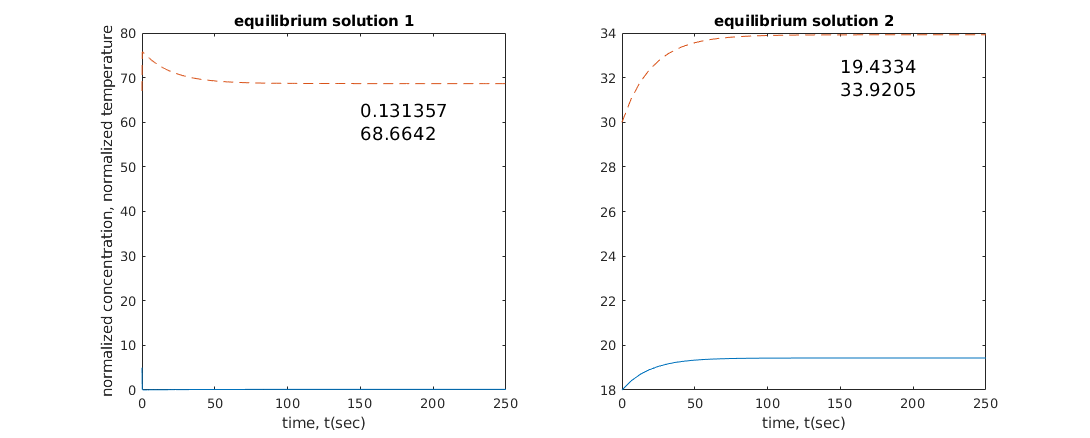
\includegraphics[width=1.1\textwidth]{../matlab/img/simu.png}
\caption{Simulation of the model}
\label{fig:simu}
\end{figure}

The equilibria are: \textbf{[0.131357, 68.6642]} and  \textbf{[19.4334, 33.9205]}.
\subsection{fminsearch function}
After having found two equilibria by simulation, we can use a ``shell'' function in order to use 
\textit{fminsearch} function:
\lstinputlisting{../matlab/mag_sq_xdot.m}
\lstinputlisting{../matlab/fminsearch_exo.m}

with results: 
\begin{align}
    x_{eq1} &= \begin{bmatrix}
        0.1314 \\
        68.6642
    \end{bmatrix} \\
    x_{eq2} &= \begin{bmatrix}
        19.4334 \\
        33.9206
    \end{bmatrix} \\
    x_{eq3} &= \begin{bmatrix}
        11.6442 \\
        47.9411
    \end{bmatrix}
\end{align}

As we can see, the first two equilibrium points are very similar to the ones we found through simulation. 
However, there is a third equilibrium that we need to analyze because it corresponds to the unstable 
equilibrium.

\section{Small Signal Linearization}
In order to linearize our model around our operating points we use the following:
\begin{align}
    A &= \left. \frac{\partial f}{\partial x} \right\rvert_{x_0, u_0} \\
    A &= \left. \begin{bmatrix}
        \frac{\partial f_1}{\partial x_1} & \frac{\partial f_1}{\partial x_2} \\ 
        \frac{\partial f_2}{\partial x_1} & \frac{\partial f_2}{\partial x_2} 
    \end{bmatrix} \right\rvert_{x_0, u_0}
\end{align}

we can define our $f_i$ functions based on our model defined in equations (\ref{eq:exo1}) and (\ref{eq:exo2}):

\begin{align}
    f_1 &= \frac{u_1 u_3}{V} - \frac{u_1 x_1}{V} - \alpha x_1 e^{-\frac{\beta}{x_2 + 46}} \\
    f_2 &= \frac{u_1 u_2}{V} - \frac{u_1 x_2}{V} - \frac{\alpha \gamma x_1}{\sigma} e^{-\frac{\beta}{x_2 + 46}}
\end{align}

then, compute the partial derivatives:

\begin{align}
    \frac{\partial f_1}{\partial x_1} &= -\frac{u_1}{V} - \alpha e^{-\frac{\beta}{x_2 + 46}} \\
    \frac{\partial f_1}{\partial x_2} &= -\frac{\alpha \beta x_1}{(x_2 + 46)^2} e^{-\frac{\beta}{x_2 + 46}} \\
    \frac{\partial f_2}{\partial x_1} &= \frac{\alpha \gamma}{\sigma} e^{-\frac{\beta}{x_2 + 46}} \\
    \frac{\partial f_2}{\partial x_2} &= -\frac{u_1}{V} + \frac{\alpha \beta \gamma x_1}{\sigma(x_2 + 46)^2} e^{-\frac{\beta}{x_2 + 46}}
\end{align}

and write a matlab function for the linearized model:
\lstinputlisting{../matlab/linear_exo.m}

\subsection{Eigen Analysis}

Once we have our linearized model around the equilibria, it is easy to find its eigenvalues and eigenvectors
to analyze the behaviour of the system using the matlab function \textit{eig}:

\lstinputlisting{../matlab/eigen_analysis.m}

\subsubsection{First Equilibrium}
In this case for the equilibrium at \textbf{[0.1314, 68.6642]}, our A matrix, eigenvalues and eigenvectors are:

\begin{align}
    A &= \begin{bmatrix}
        -7.4983 & -0.2083 \\
        13.4060 & 0.3245
    \end{bmatrix} & \\
    \lambda_1 &= -7.1233 &v_1 = \begin{bmatrix}
        -0.4856 \\0.8742
    \end{bmatrix} \\ 
    \lambda_2 &= -0.0505 &v_1 = \begin{bmatrix}
        0.0280 \\-0.9996
    \end{bmatrix}
\end{align}

from this results the following conclusions can be made:
\begin{itemize}
    \item both eigenvalues, $\lambda_1 = -7.1233$ and $\lambda_2 = -0.0505$ have \textbf{negative real part} which means that both are stable, hence, this equilibrium is \textbf{stable}.
    \item $\lambda_1$ is significantly bigger than $\lambda_2$, therefore we can say that this eigenvalue is the fast one and $\lambda_2$ the slow one.
    \item the trajectories near the first equilibrium follow the directions given by the eigenvectors $v_1$ and $v_2$. The state will follow $v_1$ faster than $v_2$ since $\lambda_1$ is the fastest eigenvalue.
\end{itemize}

\subsubsection{Second Equilibrium}
In this case for the equilibrium at \textbf{[19.4334, 33.9206]}, our A matrix, eigenvalues and eigenvectors are:

\begin{align}
    A &= \begin{bmatrix}
        -0.0507 & -0.0016 \\
        0.0003 & -0.0477
    \end{bmatrix} & \\
    \lambda_1 &= -0.0505 &v_1 = \begin{bmatrix}
        -0.9932 \\0.1166
    \end{bmatrix} \\ 
    \lambda_2 &= -0.0479 &v_1 = \begin{bmatrix}
        0.4856 \\-0.8742
    \end{bmatrix}
\end{align}

from this results the following conclusions can be made:
\begin{itemize}
    \item both eigenvalues, $\lambda_1 = -0.0505$ and $\lambda_2 = -0.0479$ have \textbf{negative real part} which means that both are stable, hence, this equilibrium is \textbf{stable}.
    \item $\lambda_1$ and $\lambda_2$ are very close in magnitude, therefore both eigenvalues are very similar in behaviour.
    \item the trajectories near the equilibrium follow the directions given by the eigenvectors $v_1$ and $v_2$. The state will follow $v_1$ and $v_2$ at very similar rate so there is no dominant direction.
\end{itemize}

\subsubsection{Third Equilibrium}
For the last equilibrium found at \textbf{[11.6442, 47.9411]}, our A matrix, eigenvalues and eigenvectors are:

\begin{align}
    A &= \begin{bmatrix}
        -0.0846 & -0.1259 \\
        0.0614 & 0.1762
    \end{bmatrix} & \\
    \lambda_1 &= -0.0505 &v_1 = \begin{bmatrix}
        -0.9653 \\0.2613
    \end{bmatrix} \\ 
    \lambda_2 &= 0.1421 &v_1 = \begin{bmatrix}
        0.4856 \\-0.8742
    \end{bmatrix}
\end{align}

from this results the following conclusions can be made:
\begin{itemize}
    \item in this case $\lambda_1$ has negative real part, however, $\lambda_2$ has \textbf{positive real part}, therefore this equilibrium is \textbf{unstable}.
    \item due to the nature of this equilibrium, the trajectories nearby follow directions that get farther from it.
\end{itemize}

\subsection{Visualization of eigenvectors}
In order to get a better understanding of the nature of the equilibria of our system, we can plot the eigenvectos located at each operating point, 
the results are shown in Figure(\ref{fig:eigenvectors}).

%%%% Figura 1 %%%%%%
\begin{figure}[!h] 
    \centering
    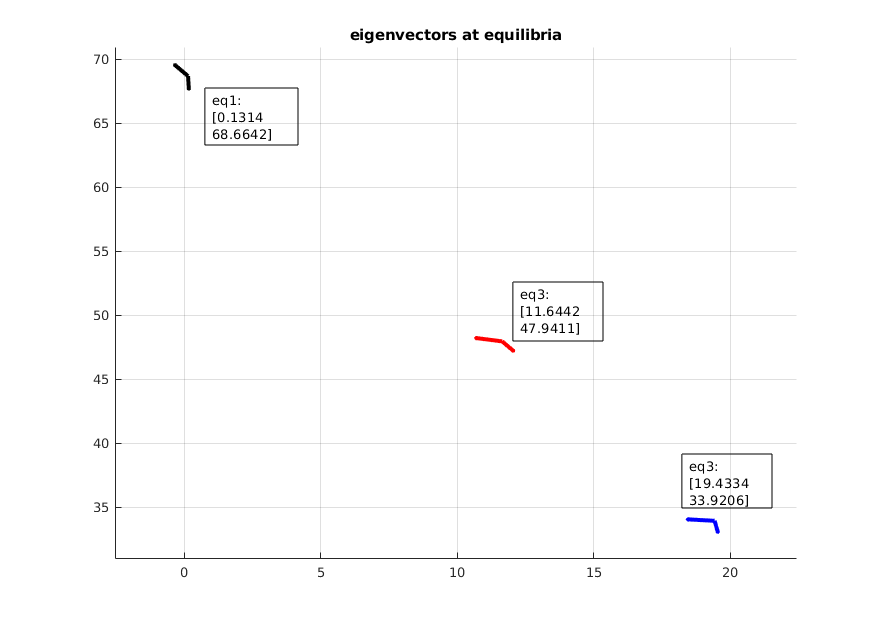
\includegraphics[width=1.1\textwidth]{../matlab/img/eigenvectors.png}
    \caption{Graphic Visualization of the system eigenvectors at equilibria}
    \label{fig:eigenvectors}
    \end{figure}
\end{document}

\subsection{Simulation of trajectories}
Once we analyzed the equilibria, and the behaviour of the system near them through eigen analysis, we can run several simulations 
for visualizing the nature of the trajectories and validate the previous results. In this case, a little routine for run 
several simulation in a loop with random initial condition has been developed, the results are shown in Figure(\ref{fig:trajectories}).

\lstinputlisting{../matlab/trajectories.m}

%%%% Figura 1 %%%%%%
\begin{figure}[!h] 
    \centering
    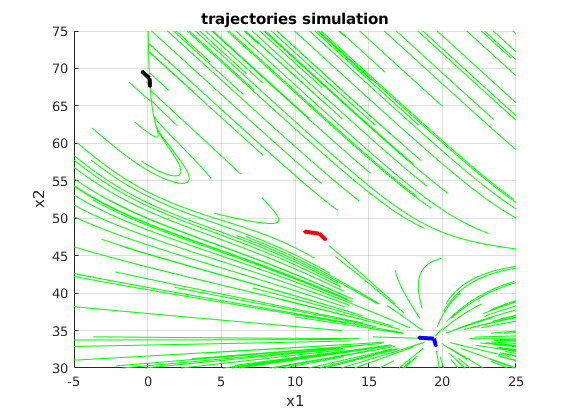
\includegraphics[width=1.1\textwidth]{../matlab/img/trajectories.png}
    \caption{Graphic Visualization of the system trajectories}
    \label{fig:trajectories}
    \end{figure}
\end{document}

For this simulation we ran 200 trajectories with random initial conditions. It is clear that the trajectories behave as we expected 
when we analyzed equilibria and eigenvalues and eigenvectors of SSL system at equilibria. 